\chapter{Problem Approach}
\label{Detailed Problem Definition}
\section{Detailed Problem Definition}
\label{sec:detailed_problem_definition}

\subsection{Motivation: From Local Forecasting to Relational Forecasting}
\label{subsec:motivation_local_relational}

Many traditional retail demand forecasting systems consider each item as a single time series. The future demand for item \( p_i \) is predicted using the historical data for that item:

\begin{equation}
    \hat{y}_{i,t+1} = f\left(y_{i,t-k:t}, X_{i,t+1}\right),
    \label{eq:local_forecasting}
\end{equation}

where \( y_{i,t-k:t} \) represents the recent past demand history for item \( p_i \), and \( X_{i,t+1} \) comprises exogenous variables (calendars, holidays, etc.) known at the time when the demand is being forecasted.

Although this formulation is suitable for modelling product-specific temporal behavior, it ignores the possible relationships between products. In retail environments, products may interact through substitution, complementarity, shared seasonality, joint promotional effects or common exposure to market trends. Therefore, modelling each product independently may discard useful contextual information available in the demand behavior of the related products.

The central motivation of this study is to investigate whether the forecasting of an individual product can be improved by incorporating information from structurally related products.

\subsection{Core Hypothesis}
\label{subsec:core_hypothesis}

The core hypothesis of this dissertation is that incorporating relational
information, derived from a dynamic item graph, improves the local forecasting of
an individual item $p_i$ relative to a purely univariate model, and Crucially,
forecasting performance is assessed along two complementary axes: the
\emph{magnitude} of the prediction error (e.g.\ MAE) and the \emph{directional}
accuracy of demand movements (for example, POCID). The hypothesis is evaluated separately
on each axis, since relational context may benefit one without benefiting --- or
while harming the other. Items are defined as vertices of the graph as
follows:
\begin{equation}
    \mathcal{G}_t = \left(\mathcal{V}, \mathcal{E}_t\right),
    \label{eq:dynamic_graph}
\end{equation}
where $\mathcal{V}$ represents the set of all items, and $\mathcal{E}_t$ denotes
time-varying relationships between the items. These relationships can be created
through various forms of statistical similarity/relationship measurements,
including but not limited to Spearman's correlation coefficient, Pearson's
correlation coefficient, Complexity Invariant Distance (CID), and other
time-series similarity measurement method. In the case of the graph presented
However, no explicit causality was established. Rather, we established a structural
framework that enables the extraction of contextually relevant information based
on the co-movements and/or behaviors of neighboring items, which would aid in
to predict the behavior of the target item.

\subsection{Dynamic Nature of Product Relationships}
\label{subsec:dynamic_product_relationships}

A key assumption of this study is that product relationships are not static. Similarities between demand series may change over time owing to promotions, seasonal effects, stock availability, changes in consumer behavior, or external shocks.

Therefore, the problem was formulated using dynamic graphs. Instead of assuming a fixed product graph for the entire forecasting period, the graph is reconstructed over the rolling historical windows. At each time step \(t\), a graph \(\mathcal{G}_t\) is built using the most recent demand observations, for example, over a window of length \(w\):

\begin{equation}
    Y_{t-w:t}.
    \label{eq:rolling_window}
\end{equation}

This allows the relational structure to reflect short-term changes in product behavior. Consequently, the forecasting problem becomes not only temporal but also spatiotemporal: the model must learn from both the historical demand of the target product and the evolving structure of its product neighborhood.

\section{Formal Problem Statement}
\label{sec:formal_problem_statement}
Based on the given data about each target product (historical demands of each product, exogenous factors, etc.) and the dynamic product graph, we want to develop an estimation method that predicts the future demand for products:

\[ \hat{ y }_{ i , t + 1} = F \left( { Y _{ i , t - k : t}, X_{ i , t + 1}, \phi \left( {\mathcal{G}}_t,i \right)} \right), \]

where $ Y _{ i , t - k : t}$ is the recent historic demand value for product $ p _i$, $ X_{ i , t + 1}$ is the forecasted value of all exogenous factors in the time step $t + 1$ and $\mathcal{G}_t$ is the graph built by us up to the time $t$. In addition, $\phi (\mathcal{G})_t,i)$ defines the structural/neighborhood features derived from the graph for product $ p _i$.

The forecasting function $ F (\cdot )$ depends on the implementation of the selected model. Graph features ($ \phi (\mathcal{G})_t,i))$ can be generated using several techniques, including but not limited to graph embeddings, neighborhood aggregation, graph convolutions, attention-based aggregation, and recurrent graph-based methods.

\subsection{Limitations of Decoupled Graph Embedding Approaches}
\label{subsec:limitations_decoupled_embeddings}

Graph information can be incorporated into an approach by generating graph or node embeddings and using them as additional feature inputs in a forecasting model, such as a long short-term memory (LSTM) network. The decoupled strategy has many limitations in dynamic forecasting environments.

The first limitation arises because the embeddings are independently computed at every time step. Consequently, the resultant vector space does not have a common alignment over time. This means that an embedding space of a given dimensionality cannot provide the same semantic representation from one graph snapshot to another. In a recursive forecasting environment, this instability makes it challenging for temporal models to identify consistent patterns.

Second, although decoupled approaches isolate the learning of representations from the goals of forecasting, they do not optimize the graph embedding model to better forecast demand. Consequently, the generated embeddings may include the structural characteristics of graphs that are not valuable to the ultimate goal of demand forecasting.

Finally, because graph-level representations (for example, Graph2Vec) may not be as well-suited to applications where demand forecasts for individual products are desired, neighborhood-level representations or node-level representations would be more appropriate for this dissertation's forecasting objective.

\subsection{Research Objectives} \label{subsec:research_objective}

The primary purpose of this research was to assess whether relational information expressed through dynamic graph-based structures could lead to improvements in local product-level forecasted demand.

Specifically, this dissertation will transition from a modular pipeline of the following form:

\begin{equation}
\text{Graph Construction} \rightarrow \text{Embedding Generation} \rightarrow \text{Forecasting Model}. \label{eq:modular_pipeline}
\end{equation}

to an integrated spatiotemporal modeling framework, where both graph-based aggregation and temporal forecasting occur simultaneously.

Examples of candidate architectures include models using GraphSAGE, Graph Attention Networks (GAT), graph convolutional network-long short-term memory hybrid (GCN-LSTM) models, and other types of dynamic graph neural networks, including EvolveGCNs. These models are applicable because they provide the ability to gather information from neighboring products and preserve the local forecasting objectives for the target product.

This type of formulation has at least three advantages.

\begin{enumerate}
\item \textbf{Inductive Processing of Dynamic Neighborhoods:} The model has the ability to use dynamically changing neighborhoods without having to create a completely new embedding space to be trained from scratch at every time step.

\item \textbf{Joint Modeling of Spatial and Temporal Dependencies:} The model can use the temporal characteristics of the target product along with the relational information gathered from its neighborhood graph.

\item \textbf{Task-Oriented Neighbor Aggregation:} Instead of assuming that all statistically similar products will be equally beneficial to the forecasting model, the model can determine what neighbors and relationships are most beneficial to the forecasting task.
\end{enumerate}


In general, this study defines the forecasting problem as a local prediction task that includes additional context regarding dynamically changing neighborhood information. The intention of this study is not to replace the existing product-specific temporal model but to add relational signals generated from product graphs as they evolve.

\subsection{Dynamic Graph Construction}
\label{subsec:dynamic_graph_construction}

The first stage of the proposed solution involves translating the multivariate product demand series into a graph structure. At each time step \(t\), a graph is constructed as follows:

\begin{equation}
    \mathcal{G}_t = \left(\mathcal{V}, \mathcal{E}_t, A_t\right),
    \label{eq:dynamic_graph_with_adjacency}
\end{equation}

where \(\mathcal{V}\) denotes the set of products, \(\mathcal{E}_t\) represents the set of edges at time \(t\), and \(A_t\) is the corresponding weighted adjacency matrix.



\subsubsection{Target-Centric Topology}

\label{subsubsec:target_centric_topology} The graph is built around the target product $p_{i}$ because the forecasting task is a local one. Here, $p_{i}$ serves as the center point of a local "neighborhood" graph with connections to other potential neighboring products. This creates a target-centric/star graph structure, where there are direct connections from the center product to the most important products relative to the chosen criteria for similarity/distance. Formally, the local graph for each product $p_{i}$ is represented at time $ t $ as follows:

\begin{equation}
    \mathcal{G}_{i,t} = \left(\mathcal{V}_{i,t}, \mathcal{E}_{i,t}\right),
    \label{eq:target_centric_graph}
\end{equation}

In \ref{eq:target_centric_graph}, $\mathcal{V}_{i,t}$ represents both the target product $p_{i}$ and its neighbor(s), and $\mathcal{E}_{i,t}$ denotes the edges that connect these neighbors to the target product.



\subsubsection{Statistical Edge Weighting}
\label{subsubsec:statistical_edge_weights}

Similarity/distance measures between products were calculated to determine the edges of this network. The similarity/distance measures are based on the statistical properties of the historical demand patterns of each product. Assume that we have two products, $p_i$ and $p_j$. Their respective historical demand patterns will be denoted by $$Y_{i,t-w:t}$$ and $$Y_{j,t-w:t}$$ The weight of the edge connecting the demand pattern for product $p_i$ with the demand pattern for product $p_j$, at time $t$, is given by

\begin{equation}
a_{ij,t}=s\left(Y_{i,t-w:t}, Y_{j,t-w:t}\right).
\label{eq:edge_weight_similarity}
\end{equation}

In (\ref{eq:edge_weight_similarity}), $s(\cdot)$ represents a function that measures the similarity of the historical demand patterns of the products. Examples include Pearson and Spearman correlations. When CID is used as a distance metric, it can be converted to a similarity score prior to determining the weights of the edges between products.

As previously mentioned, the resulting weighted graph provides a representation of the statistical comovements/behavioral similarities among the products' demand patterns. Again, as previously emphasized, while statistically significant evidence exists demonstrating that the products represented by each node exhibit empirically identifiable dependencies, there is no empirical evidence demonstrating that one product causes another; therefore, the edges represent empirically identified dependencies that potentially provide valuable predictive information.

\subsubsection{Temporal Windowing}
\label{subsubsec:temporal_windowing}

Instead of constructing a single static graph for the entire forecasting period, the framework generates a sequence of graphs using a sliding-window mechanism. At each time step \(t\), the graph is computed using the most recent \(w\) observations as follows:

\begin{equation}
    Y_{t-w:t}.
    \label{eq:sliding_window_graph}
\end{equation}

This produces the following dynamic graph sequence:

\begin{equation}
    \left\{
    \mathcal{G}_{i,1},
    \mathcal{G}_{i,2},
    \dots,
    \mathcal{G}_{i,T}
    \right\},
    \label{eq:dynamic_graph_sequence}
\end{equation}

where each graph reflects the local relational structure of the target product at a given time. This dynamic construction allows the model to account for changes in product relationships caused by seasonality, promotions, stock availability, market shifts, and other external factors.

\subsection{Relational Feature Extraction}

\label{subsec:relational_feature_extraction}

Once the dynamic graphs are built, the framework proceeds to the second stage: the extraction of structural information for each graph snapshot. Two major techniques were investigated. First, substructure-based graph embeddings were considered. Second, the application of inductive graph neural networks is explored to represent the structure of each graph snapshot.

\subsubsection{Substructure-Based Embeddings with Graph2Vec}

\label{subsubsec:graph2vec_embeddings}

The first strategy employs a technique called Graph2Vec to produce static vector representations of each graph snapshot. In essence, Graph2Vec treats each graph as an analog to a document and its rooted subgraphs as analog ``words.” Therefore, the objective is to obtain a vector representation that captures both the structural properties of the graphs and their relationships.

This process can be divided into two steps. First, the Weisfeiler-Lehman relabelling procedure is applied to extract rooted subgraph signatures from each graph. These subgraph signatures encode the local structures surrounding each node. Second, the extracted signatures are used as inputs to a learning process inspired by Doc2Vec \cite{le2014distributedrepresentationssentencesdocuments}. Typically, this learning process is based on the PV-DBOW architecture. Consequently, a static vector representation (also referred to as an embedding) was generated for each graph.

For each graph $\mathcal{G}_{i,t}$, Graph2Vec generates the following structural vector representation:

\begin{equation}
    z_{i,t}^{G2V} = \Phi_{G2V}\left(\mathcal{G}_{i,t}\right),
    \label{eq:graph2vec_embedding}
\end{equation}

where \(\Phi_{G2V}(\cdot)\) denotes the Graph2Vec embedding function.

Although this strategy provides a simple way to incorporate graph topology into a forecasting model, it has limitations in dynamic and recursive inference settings. Because embeddings may need to be recomputed as new graph snapshots are generated, the resulting vector spaces may not remain consistent over time. This can lead to embedding instability, where the meaning of each latent dimension changes across graph snapshots, making it difficult for the downstream temporal model to learn stable patterns.
\subsubsection{Inductive Graph Neural Networks}
\label{subsubsec:inductive_gnns}

Transductively trained or statically learned graph embedding models have an issue with consistency because they are separately learned for each graph.

Therefore, this study used Inductive Graph Neural Network (GNN) encoders. The primary difference between these models and those that are transductive is that inductive GNN's encode a set of common neural aggregation functions that may be used to process previously unseen, evolving graph structures using fixed model parameters.

Within the framework of this study, a GNN encoder accepts the graph structure \(A_t\) and node features \(H_t^{(0)}\) at time \(t\). Using Equation \ref{eq:gnn_layer_general}, node-level representations are generated as follows: 
\begin{equation}
H_t^{(l+1)} = 
\sigma\left(
\operatorname{AGG}^{(l)}\left(H_t^{(l)}, A_t\right)
\right).
\label{eq:gnn_layer_general}
\end{equation}

Here, $H_t^{(l)}$ represents the node representation matrix at layer $l$, $A_t$ represents the adjacency matrix associated with the sliding window topology at time $t$, $\operatorname{AGG}^{(l)}(\cdot)$ represents a learnable aggregation function, and $\sigma(\cdot)$ is a nonlinear activation function. Two different inductive GNN architectures were designed in this study to serve as the spatial encoders.


\paragraph{Graph Convolutional Networks (GCN). }

The GCN applies a localized first-order approximation to spectral graph convolutions. It uses degree-normalized adjacency matrices to gather Neighborhood Information. The layer-wise propagation rule for each layer can be expressed as follows:

\begin{equation}
    H_t^{(l+1)} =
    \sigma\left(
        \tilde{D}^{-1/2} \tilde{A}_t \tilde{D}^{-1/2} H_t^{(l)} W^{(l)}
    \right),
    \label{eq:gcn_update}
\end{equation}

with \({\tilde{A}_{t}} = {A_{t}} + {I}\) being the adjacency matrix with self-loops and \({\tilde{D}}\) its corresponding diagonal degree matrix, and \(W ^{\left(l\right)}\) being a trainable weight matrix. This enables an efficient structure-driven embedding mechanism that smoothly transfers features across the connected products.

\paragraph{Graph Attention Networks (GAT).}
A major distinction between GCNs and Graph Attention Networks (GATs) is the method used to produce node aggregation weights for a node. In the case of GCNs, this process relies on the structural relationship between all nodes concerning their degrees. In contrast, in GATs, a learned weighting scheme utilizes the similarity of each neighbor vector representation to dynamically create a weighting scheme from all neighbors. The new representation of node v for layer l + 1 can be represented by the following equation:

\begin{equation}
h_v^{(l+1)}=
\sigma \left (
\sum _{ u \in \mathcal { N } ( v ) \bigcup \{ v \}} 
\alpha _{{ v , u }}^{\left( l \right) } W ^ {\left( l \right) } h_{{ u }}^{\left( l \right) }
\right ),
\label{eq:gat_update}
\end{equation}

where \(\mathcal { N }( v )\) represents the neighborhood of \(v\), and \(\alpha _{{ v , u }}^{\left( l \right) }\) is an attention weight generated through a learned mechanism as a function of the features of nodes \(u\) and \(v\). As part of the process of ensuring that the training of GAT networks is stable, all GAT layers utilize multi-head attention. Multi-head attention involves concatenating the results of K separate attention operations in the hidden layer of the network. This allows the model to learn about different types of relational behavior, for example, which neighbors may have experienced real demand shifts versus those that have been subject to noise.

Both the GCN and GAT encoders extract structural representations for each target product p i at time t from the rows in the resulting output matrix from the last layer:

\begin{equation}
z_{{ i , t }}^ {{ GNN }}=h_{{ i , t }}^{{ L }},
\label{eq:target_node_embedding}
\end{equation}

Where L represents the final layer of the GNN. Thus, the encoder applies the same shared parameters to every window, projecting a sequence of dynamic graphs onto a stable, consistent latent space, so that the temporal head can consume the embedding of any window without modification despite the changing topology.

\subsection{Architecture General Overview}
\label{subsec:architecture_general_overview}

An integrated, dual-branch architecture was developed in which graph-derived
structural representations are fused with the sequential forecast generation and
trained \emph{end-to-end} with the temporal model under a single forecasting loss
(in contrast to the embedding-decoupled Graph2Vec pipeline of
Section~\ref{subsubsec:graph2vec_embeddings}). At each time step, the temporal model takes as input the
dynamic relational structure in which the target product exists in the market.


\begin{figure}[htbp]
    \centering
    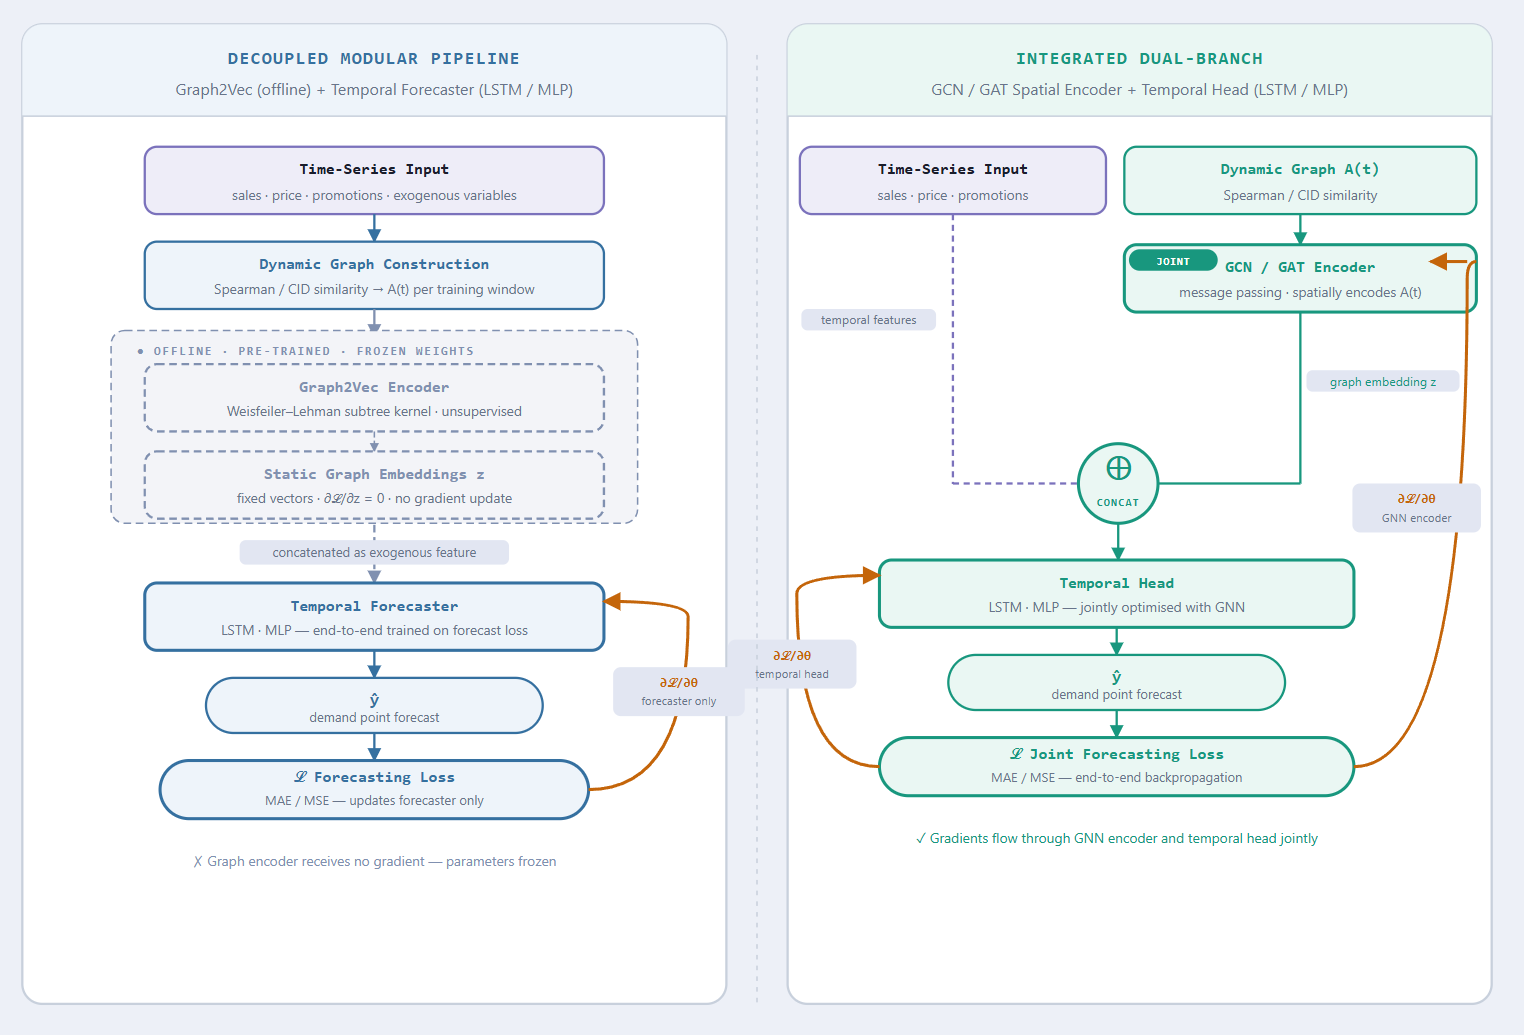
\includegraphics[width=\textwidth]{figures/decoupled_vs_integrated.png}
    \caption{Conceptual comparison of the two relational forecasting paradigms evaluated in this study. The left panel illustrates the decoupled modular pipeline (Graph2Vec), where the graph representations are learned offline. The right panel depicts the proposed integrated dual-branch architecture, where the spatial GNN encoder and temporal head are optimized jointly end-to-end via a single forecasting loss. (\textit{Note: This diagram was generated with the assistance of Claude Sonnet}).}
    \label{fig:pipeline_comparison}
\end{figure}


For each time step t in the sequence, the temporal model processes the concatenated input vector as follows:
\begin{align*}
u_{i,t}&=
CONCAT(y_{i,t},X_{i,t},z_{i,t}^{GNN})
\label{eq:temporal_input_concat}.
\end{align*}

Here,
$y_{i,t}$ represents the historical demand for the target item; $X_{i,t}$ includes other variables, such as promotional activities and seasonal factors; and $z_{i,t}^{GNN}$ represents the spatial contextual information from the GCN or GAT encoder.

To process this augmented sequence and capture the temporal dynamics, two distinct temporal architectures were evaluated:

\paragraph{LSTM Forecaster.}
The Long Short-Term Memory (LSTM) network processes the sequence iteratively, updating a hidden state that maintains a continuous memory of the product's trajectory and shifting relational context:
\begin{equation}
    h_{i,t}^{LSTM} =
    \operatorname{LSTM}
    \left(
        u_{i,t},
        h_{i,t-1}^{LSTM}
    \right).
    \label{eq:lstm_hidden_state}
\end{equation}
The final prediction is extracted by passing the hidden state from the most recent sequence step through a linear output head: \(\hat{y}_{i,t+1} = W_{out} \cdot h_{i,T}^{LSTM} + b_{out}\).

\paragraph{Time-Distributed MLP Forecaster.}
As an alternative to the recurrent constraints of the LSTM, a Time-Distributed Multilayer Perceptron (MLP) applies a shared set of feed-forward layers independently to every step in the lookback window:
\begin{equation}
    h_{i,t}^{MLP} =
    \operatorname{MLP}_{shared}
    \left(
        u_{i,t}
    \right).
    \label{eq:mlp_timestep}
\end{equation}
To aggregate the temporal sequence into a single context vector without recurrence, the model pools time-distributed outputs. Specifically, the latest state is concatenated with the global average across the window before being mapped to the forecast horizon as follows:
\begin{equation}
    \hat{y}_{i,t+1} =
    W_{out} \cdot 
    \operatorname{CONCAT}
    \left(
        h_{i,T}^{MLP}, 
        \frac{1}{T}\sum_{t=1}^{T} h_{i,t}^{MLP}
    \right)
    + b_{out}.
    \label{eq:mlp_output_prediction}
\end{equation}

This dual-branch design ultimately yields four distinct spatiotemporal permutations (GCN-LSTM, GCN-MLP, GAT-LSTM, and GAT-MLP), enabling a rigorous comparison of how different aggregation mechanisms and temporal processors leverage dynamic retail graphs to predict future sales.

\subsubsection{Recursive Inference}
\label{subsubsec:recursive_inference}

To predict future steps in time (multi-step-ahead forecasting), the model employs a "recursive" approach to make new predictions. Once we have made our prediction of \(\hat{y}_{i,t+1}\), that prediction becomes part of our input data at the next step. Therefore, we can write this recursive forecasting process as

\begin{equation}
\hat{y}_{i,t+h} = 
F\left( \hat{Y}_{i,t:t+h-1}, 
X_{i,t+h},
z_{i,t+h-1} \right)
, \label{eq:recursive_forecasting}
\end{equation}

where h represents how far ahead forecasts are made with respect to the current time t. In addition, \(\hat{Y}_{i,t:t+h-1}\) refers to all previously generated predictions that will be used as inputs for the next forecast.

In a dynamic graph framework, the graph can be modified while recursively generating forecasts. When using the predicted values from the target product, we can modify the demand history. Crucially, only the focal item's row of this window is supplied by the model's own predictions; every other product contributes its real observed demand over the same interval. This provides a mechanism by which the graph structure evolves over the course of the inference process, reflecting both the most recent estimate of the state of the target product and its neighbors.

\subsection{Expected Contribution of the Proposed Framework} 
\label{subsec:expected_contribution_framework}

Using graph-determined relational knowledge as an input to the LSTMs allows the model to modify its immediate forecast based on the structural context of the product. Specifically, the graph structure may enable the model to determine whether a product's neighborhood is experiencing growth, decline, substitution effect, complementary behavior, or stability.

Thus, this proposed framework differs from purely localized forecasting models because it does not depend solely on the historical trajectory of the specific target product; instead, it combines the local time-series signal with dynamic relational knowledge derived from the surrounding (neighborhood) products.

\subsection{Local Focus via Global Context}
One of the distinguishing features of this method is the asymmetry with respect to the input data required by the model versus the output prediction provided by the model. The model operates on a "local" scale, attempting to optimize forecasts for each individual target item $p_i$. However, because the model must consider the influences of a dynamic graph, there will be a much larger computational scope than local.
To keep the dynamic graph $\mathcal{G}_t$ valid throughout the recursive inference, there is an ideal situation in which the system can produce a forecast for each of the other neighboring items simultaneously. This is true because the edges of the graph (CID or Spearman distance) are based on the future value of all neighbors to remain current. Local Predictive Focus: Nevertheless, despite processing numerous products to identify the "movement of the market,” the primary goal remains improving the local forecast for the target item. The auxiliary forecasts of neighboring items provide "structural support" to supply the necessary signals for updating the graph's topology and thereby enhance the quality of the target item's prediction. Resource Efficiency: This distinction provides an opportunity for resource-efficient strategies. That is, while many products can be processed to capture a sufficient signal to update the topology of the graph and thus enhance the quality of the target item prediction.